 \input ../SlidePreamble
\input ../preamble


\begin{document}

{\Huge

  \centerline{\bf TTIC 31230, Fundamentals of Deep Learning}
  \bigskip
  \centerline{David McAllester, Winter 2019}
  \vfill
  \centerline{Latent Variable Models}
  \vfill
  \centerline{Expectation Maximization (EM)}
  \vfill
  \centerline{The Evidence Lower Bound (the ELBO)}
  \vfill
  \centerline{Variational Autoencoders (VAEs)}
  \vfill
  \vfill

\slide{Latent Variable Models}

We are often interested in models of the form

\vfill
{\color{red} $$P_\Phi(y) = \sum_z\;P_\Phi(z)P_\Phi(y|z)$$}
{\color{red} $$P_\Phi(y|x) = \sum_z\;P_\Phi(z|x)P_\Phi(y|z)$$}

\vfill
Here {\color{red} $z$} is the latent variable.

\slide{Reasons for Latent Variables}

\begin{itemize}
\item Measuring cross entropy.

\vfill
\item Inserting domain knowledge.

\vfill
\item Improving interpretability.
\end{itemize}

\slide{Dangers of Latent Variables}

\centerline{Domain ``knowledge'' is often wrong.}

\slide{Measuring Cross Entropy (TZ)}

For structured label spaces (sentences or images), cross-entropy is currently only measured for ``autoregressive'' (directed) graphical models.

\vfill
For images this is done with ``pixel RNNs''.

\vfill
But compression models can be viewed as latent variable models with measurable cross-entropy.

\slide{Cross Entropy of a Compression Model}

A compression model $\Phi$ maps a label $y$ to a latent value (code) $z_\Phi(y)$ such that
there exists a decompression algorithm $y_\Phi(z)$ satisfying
{\color{red} $$y_\Phi(z_\Phi(y)) = y.$$}

\vfill
Let {\color{red} $|z_\Phi(y)|$} be the bit length of the compression of $y$.

\slide{Cross Entropy of a Compression Model}

{\color{red}
\begin{eqnarray*}
\Phi^* & = & \argmin_\Phi \;E_{y \sim \pop} \;-\ln P_\Phi(y) \\
& = & \argmin_\Phi \;E_{y \sim \pop} \;|z_\Phi(y)|
\end{eqnarray*}
}

\vfill
Assuming universal expressive power, Shannon's source coding theorem implies

{\color{red} $$E_{y \sim \pop}\; |z_{\Phi^*}(y)| \leq H_2(y) +1$$}

\slide{Measuring Rate-Distortion Points}

A noisy-channel RDA

{\color{red}
\begin{eqnarray*}
\Phi^* & = & \argmin_\Phi I(y,z) + \lambda E_{y \sim \pop,\;z\sim p_\Phi(z|y)}\; \mathrm{Dist}(y,y_\Phi(z))
\end{eqnarray*}
}

has a measurable rate-distortion trade off provided we can measure the bandwidth {\color{red} $I(y,z)$} of the noisy channel.

\slide{Sparse Labeling Compression (TZ)}

Given a graphical model $\Phi$ on semantic segmentations we can code a segmentation $y$
by a sparse segmentation {\color{red} $z_\Phi(y)$} assigning a label to only a small fraction of the pixels.

\vfill
We can define a decoding {\color{red} $y_\Phi(z)$} to be the result of running a deterministic local search over
the labels of the unspecified pixels to find a locally best-scoring full semantic segmentation.

\vfill
We can then define the encoding {\color{red} $z_\Phi(y)$} to be
$${\color{red} z_\Phi(y)} = \argmin_{z:\; {\color{red} y_\Phi(z) = y}}\;|z|$$
where $|z|$ is the number of pixels assigned by $z$.

\slide{Encoding Domain Knowledge}

In CTC the latent variable $z$ (the latent sequence of phonemes and blanks) and the blank removal operation $y(z)$ constitute useful engineered domain knowledge.

\vfill
There have been many attempts to build standard latent linguistic structure, such as parse trees, into deep language models.  These attempts have
largely failed to improve performance on end-to-end applications.

\vfill
Attempts to use classical graphical models in computer vision have also largely failed.

\vfill
But I believe that we should not give up on engineering.

\slide{Improved Interpretabilty}

In CTC we can see where in the input signal system the gold labels are coming from.

\vfill
If we have latent parse trees in an NLP model we can see what parse the system is using.

\vfill
If the latent variables are engineered to have semantics then, by construction, we have a semantic interpretation of internal processing.

\slide{Attention and Latent Variables}

In machine translation attention is used to handle a latent alignment between the input sentence and the gold label translation.

\vfill
In general, attention can be viewed as defining a probability distribution over a latent choice.

\vfill
Attention is the central mechanism in the transformer network (to be discussed later).

\vfill
The transformer network can be viewed as constructing latent trees over an input sentence.

\slidetwo{Expectation Maximization (EM)}
{Mixture of Gaussian Modeling}

{\color{red} $$\Phi = \pi[z],\mu[z],\Sigma[z],\;\;\;z \in \{1,\ldots,k\}$$}

\begin{eqnarray*}
p_\Phi(y) & = & {\color{red} \sum_z\;P(z)p(y|z)} \\
\\
& = & \sum_{z=1}^k\;\pi[z]\;\frac{1}{Z[z]}\exp\left(-\frac{1}{2}(y-\mu[z])^\top \Sigma[z]^{-1}(y - \mu[z])\right)
\end{eqnarray*}

\slidetwo{Expectation Maximization (EM)}
{Mixture of Gaussian Modeling}
\vspace{-4ex}
$$\Phi = \pi[z],\mu[z],\Sigma[z],\;\;\;z \in \{1,\ldots,k\}$$
$$\mbox{Train} = \{y_1,\ldots,y_N\}$$
Until Convergence:
$$P_\Phi(z|y_j) = \frac{\pi[z]P(y_j|z)}{\sum_z\;\pi[z]P(y_j|z)} \;\;\mbox{\color{red} Inference (E step)}$$

$$\left.
\begin{array}{rcl}
  \pi^{t+1}[z] & = & \frac{1}{N}\; \sum_j \;P_{\Phi^t}(z|y_j) \\
  \mu^{t+1}[z] & = & \frac{1}{N}\; \sum_j \;P_{\Phi^t}(z|y_j)y_j \\
  \Sigma^{t+1}[z] & = & \frac{1}{N}\; \sum_j P_{\Phi^t}(z|y_j)y_jy_j^\top
\end{array}
  \right\} \mbox{\color{red} Model Update (M step)}$$

\slide{General EM}
{\color{red} $$\Phi^* = \argmin_\Phi E_{y \sim \mathrm{Train}} -\ln P_\Phi(y)$$}

\vfill
{\color{red} $$P_\Phi(y) = \sum_z\;P_\Phi(z)P_\Phi(y|z).$$}

\vfill
$${\color{red} \Phi^{t+1}} =  {\color{red} \argmin_\Phi}\;E_{y \sim \mathrm{Train}} \;E_{z \sim {\color{red} P_{\Phi^t}(z|y)}}\; - \ln P_{\color{red} \Phi}(z,y)$$
\centerline{\hspace{1em} Update \hspace{6em} Inference \hspace{2.5em}~}
\centerline{(M Step) \hspace{5em} (E Step) \hspace{1.5em}~}


\anaslide{Colorization}
\medskip
\centerline{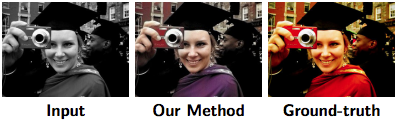
\includegraphics[width = 5in]{../images/colorizationGreg2}}
\centerline{$x$ \hspace{4em} $\hat{y}$ \hspace{4em} $y$}
\centerline{\huge Larsson et al., 2016}

\vfill
$x$ is a grey level image.

\vfill
$y$ is a color image drawn from $\pop(y|x)$.

\vfill
$\hat{y}$ is an arbitrary color image.

\vfill
$P_\Phi(\hat{y}|x)$ is the probability that model $\Phi$ assigns to the color image $\hat{y}$ given grey level image $x$.

\anaslide{Colorization with Latent Semantic Segmentation (TZ)}
\medskip
\centerline{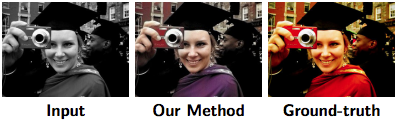
\includegraphics[width = 5in]{../images/colorizationGreg2}}
\centerline{$x$ \hspace{4em} $\hat{y}$ \hspace{4em} $y$}

\vfill
{\color{red} $$P_\Phi(\hat{y}|x) = \sum_z\;P_\Phi(z|x)P_\Phi(\hat{y}|z,x).$$}
\begin{eqnarray*}
\mbox{input}\; x \\
P_\Phi(z|x) & = & \ldots \;\;\mbox{\color{red} semantic segmentation} \\
P_\Phi(\hat{y}|z,x) & = & \ldots \;\;\mbox{\color{red} segment colorization} \\
\end{eqnarray*}

\slide{Maybe EM?}

{\color{red} $$P_\Phi(y) = \sum_z\;P_\Phi(z)P_\Phi(y|z).$$}

$${\color{red} \Phi^{t+1}} =  {\color{red} \argmin_\Phi}\;E_{y \sim \mathrm{Train}} \;E_{z \sim {\color{red} P_{\Phi^t}(z|y)}}\; - \ln P_{\color{red} \Phi}(z,y)$$
\centerline{\hspace{1em} Update \hspace{6em} Inference \hspace{2.5em}~}

\vfill
{\color{red} In most cases the inference is intractible!}

\slidetwo{Variational Inference:}
{The Evidence Lower Bound (The ELBO)}
We introduce a friendly model {\color{red} $P_\Psi(z|y)$} to approximate {\color{red} $P_\Phi(z|y)$}.

{\huge
\begin{eqnarray*}
        \ln P_\Phi(y) & = & E_{\color{red} z \sim P_\Psi(z|y)} \ln P_\Phi(y) \\
\\
 & = & E_{z \sim P_\Psi(z|y)} \left(\ln P_\Phi(y)\frac{P_\Phi(z|y)}{P_\Psi(z|y)} + \ln \frac{P_\Psi(z|y)}{P_\Phi(z|y)}\right) \\
 \\
  & = & \left(E_{z \sim P_\Psi(z|y)} \ln \frac{P_\Phi(z,y)}{P_\Psi(z|y)}\right) + KL(P_\Psi(z|y),P_\Phi(z|y)) \\
  \\
  & = & \hspace{4em} \mathrm{\color{red} ELBO} \hspace{4em}  + KL(P_\Psi(z|y),P_\Phi(z|y))
\end{eqnarray*}
}

\slide{Optimization of the ELBO}

\begin{eqnarray*}
\ln P_\Phi(y) & \geq & \mathrm{ELBO}(\Phi,\Psi,y) \\
\\
& = & E_{z \sim P_\Psi(z|y)}\;\ln\frac{P_\Phi(z,y)}{P_\Psi(z|y)}
\end{eqnarray*}

\begin{eqnarray*}
\Phi^*, \Psi^* & = & {\color{red} \argmax_{\Phi,\Psi}}\; E_{y \sim \pop}\;\mathrm{ELBO}(\Phi,\Psi,y) \\
\\
\Phi^*, \Psi^* & = & \argmax_{\Phi,\Psi}\;E_{y \sim \pop}\;{\color{red} E_{z \sim P_\Psi(z|y)}\;\ln \frac{P_\Phi(z,y)}{P_\Psi(z|y)}}
\end{eqnarray*}

\slide{EM is Alternating Maximization of the ELBO}

\begin{eqnarray*}
\mathrm{ELBO} & = & E_{z \sim P_\Psi(z|y)}\; \ln \frac{P_\Phi(z,y)}{P_\Psi(z|y)}\;\;\;(1) \\
 \\      
  & = &\ln\;P_{\Phi}(y) - KL(P_\Psi(z|y),P_{\Phi}(z|y))\;\;\;\;\;\;(2)
  \end{eqnarray*}

\vfill
\begin{eqnarray*}
\mbox{by (2)}\;\;\;\Psi^{t+1} & = & \argmin_\Psi \;E_{y \sim \mathrm{Train}} \; KL(P_{\Psi}(z|y),P_{\Phi^t}(z|y)) {\color{red} = \Phi^t} \\
\\
\mbox{by (1)}\;\;\;{\color{red} \Phi^{t+1}} & = & \argmax_{\color{red} \Phi} E_{y \sim \mathrm{Train}} \;E_{z \sim P_{\color{red} {\Phi^t}}(z|y)}\; \ln P_{\color{red} \Phi}(z,y)
\end{eqnarray*}

\slide{Hard ELBO}
\vfill
In hard EM we use only the single most likely $z$ rather than the expectation of $z \sim P_{\Phi^t}(z|y)$.

\vfill
$K$-means is hard EM for mixtures of Gaussians (when all covariances matrices are fixed at $I$).

\begin{eqnarray*}
\mathrm{ELBO} & = & \left(E_{z\sim P_\Psi(z|y)} \;\ln \frac{P_\Phi(z,y)}{P_\Psi(z|y)}\right) \\
\\
\mbox{ELBO} & = & \left(E_{z\sim P_\Psi(z|y)} \;\ln P_\Phi(z,y)\right) + H(P_\Psi(z|y)) \\
\\
{\color{red} \mbox{hard ELBO}} & {\color{red}  =} & {\color{red}  E_{z \sim P_\Psi(z|y)} - \ln P_\Phi(z,y)}
\end{eqnarray*}

\slide{A VAE for Images}

Auto-Encoding Variational Bayes, Diederik P Kingma, Max Welling, 2013.

\vfill
$${\color{red}y \hspace{5em}  z_\Psi(y,\epsilon) \hspace{4em} z\;p_\Phi(z) \hspace{3em} \hat{y}_\Phi(z) \hspace{3em}||y - \hat{y}||^2}$$
\centerline{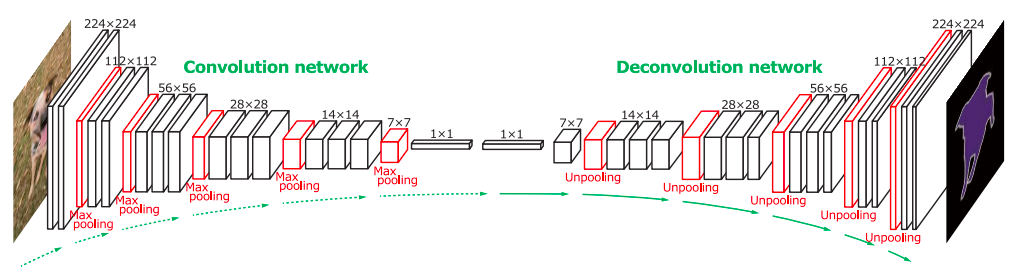
\includegraphics[width=9in]{../images/Deconv}}

\centerline{\Large [Hyeonwoo Noh et al.]}

\slide{Gaussian VAEs}

\begin{eqnarray*}
p_\Phi(z) & \propto & \exp\left(\sum_i \;(z[i] - {\color{red} \mu[i]})^2/(2{\color{red} \sigma[i]}^2)\right) \\
\\
p_\Phi(y|z) & \propto & \exp\left(\sum_j\;(y[j] - {\color{red} y_\Phi(z)[j]})^2/(2{\color{red} \gamma[j]}^2)\right) \\
\\
p_\Psi(z|y) & \propto & \exp\left(\sum_i (z[i] - {\color{red} z_\Psi(y)[i]})^2/(2{\color{red} \sigma_\Psi(y)[i]}^2)\right)
\end{eqnarray*}

\slide{Gaussian VAEs}

\begin{eqnarray*}
\mathrm{ELBO} & = & E_{z \sim p_\Psi(z|y)} \ln \frac{p_\Phi(z,y)}{p_\Psi(z|y)} \\
\\
{\cal L}_{\mathrm{ELBO}} & = & - \mathrm{ELBO} \\
\\
& = & {\color{red}  KL(p_\Psi(z|y),p_\Phi(z)) + E_{z \in p_\Psi(z|y)} - \ln p_\Phi(y|z)}
\end{eqnarray*}

\vfill
Continuous KL-divergence is ok.

\vfill
Continuous cross-entropy has issues ...

\slide{Gaussian VAEs vs. Gaussian RDAs}

\begin{eqnarray*}
{\cal L}_{\mathrm{ELBO}}(y) & = & {\color{red}  KL(p_\Psi(z|y),p_\Phi(z)) + E_{z \in p_\Psi(z|y)} - \ln p_\Phi(y|z)} \\
\\
{\cal L}_{\mathrm{RDA}}(y) & = & {\color{red}  KL(p_\Phi(z|y),p_\Psi(z)) + \lambda \; E_{z \in p_\Phi(z|y)}\; D(y,y_\Phi(z))}
\end{eqnarray*}

\vfill
Through a reparameterization these can be written as

\begin{eqnarray*}
{\cal L}_{\mathrm{ELBO}}(y) & = & {\color{red}  KL(p_\Psi(z|y),{\cal N}(0,I)) + E_{z \in p_\Psi(z|y)} - \ln p_\Phi(y|z)} \\
\\
{\cal L}_{\mathrm{RDA}}(y) & = & {\color{red}  KL(p_\Phi(z|y),{\cal N}(0,I))) + \lambda\;E_{z \in p_\Phi(z|y)}\; D(y,y_\Phi(z))}
\end{eqnarray*}

\slide{Sampling}

\centerline{Sample {\color{red} $z \sim {\cal N}(0,I)$} and compute {\color{red} $y_\Phi(z)$}}

\vfill
\centerline{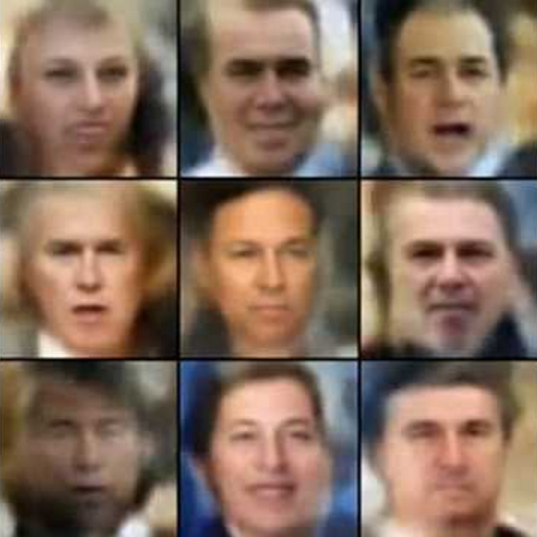
\includegraphics[width = 4in]{../images/VariationalFaces}}
\centerline{[Alec Radford]}

\slide{Reasons for Latent Variables}

\begin{itemize}
\item Measuring cross entropy.

\vfill
\item Inserting domain knowledge.

\vfill
\item Improving interpretability.
\end{itemize}

\slide{Dangers of Latent Variables}

\centerline{Domain ``knowledge'' is often wrong.}

\slide{END}


}
\end{document}

\slide{Another Way of Writing the ELBO}
{\huge
\begin{eqnarray*}
        \ln P_\Phi(y) & \geq & E_{z \sim P_\Psi(z|y)} \ln \frac{P_\Phi(z,y)}{P_\Psi(z|y)}\;\;\;\mbox{\color{red} ELBO} \\
        \\
        & = & E_{z \sim P_\Psi(z|y)} \ln \frac{P_\Phi(z)P_\Phi(y|z)}{P_\Psi(z|y)} \\
        \\
        & = & E_{z \sim P_\Psi(z|y)} \left(\ln \frac{P_\Phi(z)}{P_\Psi(z|y)} +\ln P_\Phi(y|z)\right) \\
        \\
        & = & {\color{red} \left(E_{z \sim P_\Psi(z|y)} \ln P(y|z)\right) - KL(P_\Psi(z|y),P_\Phi(z))}
\end{eqnarray*}
}

\slidetwo{Variational Inference:}
{The Evidence Lower Bound (The ELBO)}

$$P_\Phi(y) = \sum_z\;P_\Phi(z)P_\Phi(y|z)\;\;\mbox{\color{red} unfriendly composition of friendlies}$$

\begin{eqnarray*}
\ln P_\Phi(y) & = & \mathrm{ELBO} + KL(P_\Psi(z|y),P_\Phi(z|y))
\end{eqnarray*}


\vfill
{\color{red} If the friendly $P_\Psi(z|y)$ can match the unfriendly $P_\Phi(z|y)$ then the ELBO is exact.}


\slide{Hard ELBO and Rate-Distortion Autoencoding}

\begin{eqnarray*}
{\cal L}_{\mathrm{HELBO}}(y,\Phi,\Psi) &  = &  E_{z \sim P_\Psi(z|y)} - \ln P_\Phi(z,y)
\end{eqnarray*}


\vfill
{\color{red} $$\min_{P,Q} E_{y \sim \mathrm{Pop}}\;{\cal L}_{\mathrm{HELBO}}(y,P,Q) \leq H(\mathrm{Pop}) + \ln 2$$}

\vfill
This can be proved from Shannon's source coding theorem where $z$ is the code for $y$.


\slide{Measuring the ELBO}

$$\mathrm{ELBO}  =  E_{z \sim P_\Psi(z|y)}\; \ln \frac{P_\Phi(z,y)}{P_\Psi(z|y)}$$

\vfill
If $P_\Phi(z)$, $P_\Phi(y|z)$, and $P_\Psi(z|y)$ are friendly (even when $P_\Phi(y)$ is not friendly) we can
measure ELBO loss through sampling.

\vfill
If we can measure it, we can do gradient descent on it (but perhaps with difficulty).


\slide{We want $\Psi$ to adapt to $\Phi$}

$${\cal L}_{\mathrm{ELBO}}(y,\Phi,\Psi) = KL(P_\Psi(z|y),P_{\Phi}(z|y)) - \ln\;P_{\Phi}(y)$$

\vfill
$${\color{red} Q^*(z|y) = P_\Phi(z|y)}$$

\vfill
$$E_{y \sim \mathrm{Pop}}\;{\cal L}_{\mathrm{ELBO}}(y,\Phi,Q^*) = H(\mathrm{Pop},P_\Phi)$$

\slide{However, $\Phi$ can ignore $\Psi$}

$${\cal L}_{\mathrm{ELBO}}(y,\Phi,\Psi) = KL(P_\Psi(z|y),P_{\Phi}(z|y)) - \ln\;P_{\Phi}(y)$$

$${\color{red} P^*(z) = P_\Psi(z)}$$
$${\color{red} P^*(y|z) = P_\Phi(y)}$$

$$E_{y \sim \mathrm{Pop}}\;{\cal L}_{\mathrm{ELBO}}(y,P^*,\Psi) = H(\mathrm{Pop},P_\Phi)$$

\vfill
It seems important that $P_\Phi(y|z)$ have limited expressive power.




